
\chapter{Stabilization of Rabi oscillations: experimental setup}
\label{c:qfb}

With superconducting qubits, circuit QED, and nearly-quantum-limited parametric amplifiers in hand, we have all the tools needed to implement a quantum control protocol: namely, the stabilization of coherent Rabi oscillations of a qubit.  In this chapter I will describe the important aspects of the apparatus specific to the quantum feedback experiment; for excellent descriptions of the many important details in a general cQED apparatus, I refer the reader to Slichter's thesis \cite{slichterthesis} and Weber's thesis \cite{Weber2014a}.  The apparatus used for this experiment is a direct descendent from the setup described in Slichter's thesis, with relatively minimal modifications.  The weak dispersive regime of cQED---the relevant regime for this quantum feedback experiment---is also the basis for the experiments described in Weber's thesis.

\section{Relevant circuit QED parameter regime}

The scheme for demonstrating feedback control is explicitly an analog, continuous-time technique, which intrinsically creates an important hierarchy of rates in the cQED system and measurement apparatus.  We desire to create pure, sinusoidal Rabi oscillations of the qubit state, which implies that the Rabi rotation frequency $\Omega_r$ should be the fastest continuous rate in the system.  The time scale over which a measurement projects the qubit state should be much longer than one period of these oscillations, implying $\Gamma_m \ll \Omega_r$.  To ensure reliable operation of the feedback technique, we require that the rates corresponding to spontaneous relaxation and dephasing of the qubit are small compared to the measurement rate, $(\Gamma_1, \Gamma_\mathrm{env}) \ll \Gamma_m$.

Furthermore, since the feedback technique stabilizes the phase of qubit oscillations in a single plane through the Bloch sphere, we require that the back-action of the measurement correspond only to disturbances in the phase of this oscillation, not in any rotations of the qubit state in the equatorial plane.  As discussed previously in section \ref{s:cQED_backaction}, this implies that we should work in the limit of small phase shift, $2 \chi \ll \kappa$, and selectively measure only the signal quadrature containing qubit state information.  Satisfying $2 \chi \ll \kappa$ is straightforward by making the qubit-cavity coupling rate $g$ relatively small and the qubit-cavity detuning $\Delta$ relatively large.  To selectively measure the signal quadrature containing qubit state information, we use a LJPA operating in a phase-sensitive mode and align the amplification axis to this quadrature.  The result is that the photon number fluctuations in the cavity are squeezed, implying no measurement-induced pure dephasing of the qubit state due to the lack of photon number fluctuations.  This ensures that the measurement back-action does not cause the qubit state to diverge from the relevant plane of the Bloch sphere, allowing for an efficient single-parameter feedback.

\section{Experimental setup}

\begin{figure*}
\begin{center}
	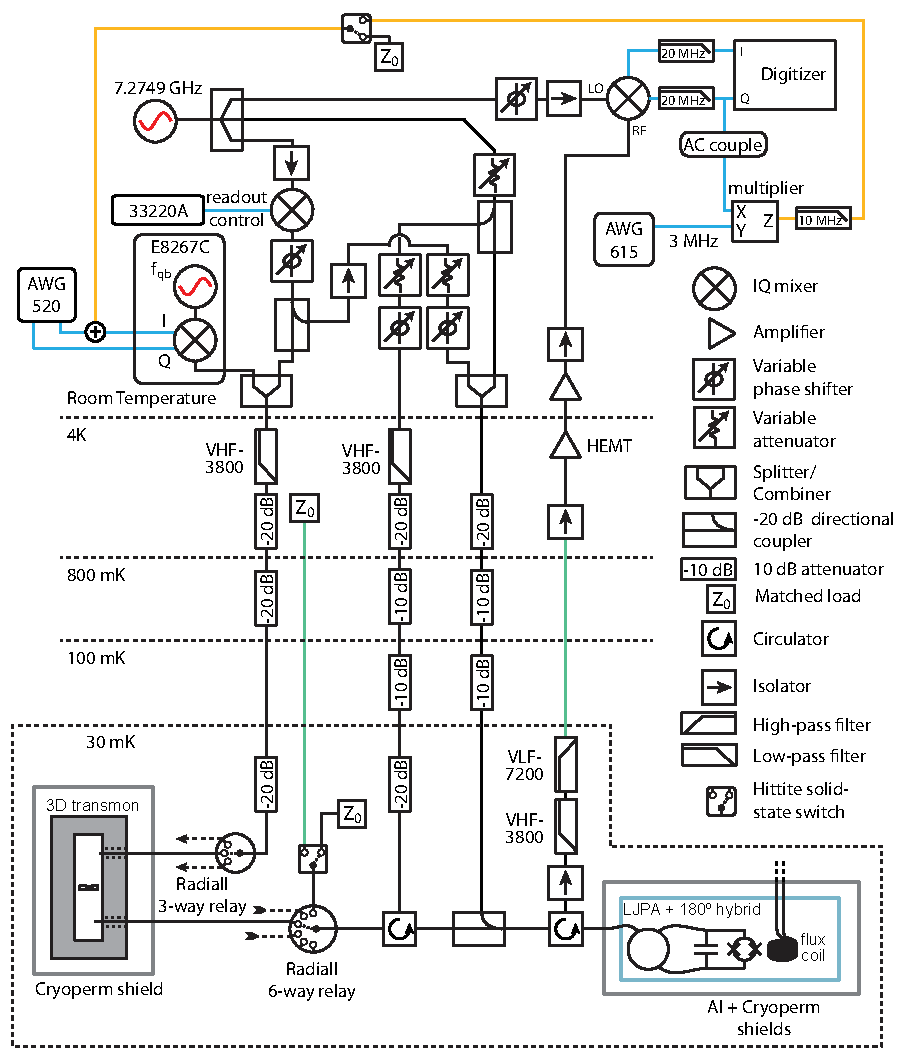
\includegraphics[width = 6in]{qfb_exp_chapter/full_schematic}
\end{center}
\caption[Experimental setup for quantum feedback]{Experimental setup for quantum feedback experiment.  Microwave signals paths are drawn as black lines, low-frequency signal paths are light blue, and the feedback error signal is drawn as an orange line.  The exception to this rule are the segments of low-loss superconducting coax lines linking 4K and 30 mK, drawn as green lines.}
\label{fig:full_schem}
\end{figure*}

A fairly complete schematic of the experimental setup for the feedback experiment is shown in Figure \ref{fig:full_schem}.  The primary missing element not shown is the trigger cascade used to control the timing in the experiments; however, the exact trigger configuration is not entirely constant across different experiments and is not as important as the signal routing.  Also omitted are low-frequency cryogenic control lines, as they are mostly used for DC biasing and are not changed during a particular experimental run.

\subsection{Qubit and parametric amplifier}

At the bottom of Figure \ref{fig:full_schem}, the primary elements of interest are the 3D transmon qubit system, at left, and the LPJA (paramp), at right.  The 3D transmon consists of a single-junction transmon qubit with transition frequencies $\omega _{01}/2\pi =5.4853$ GHz and $\omega _{02}/2\pi =10.7382$ GHz. From these values, we calculate $E_J=19.274$ GHz and $E_C=0.211$ GHz giving $E_J/E_C = 91$.  The transmon is fabricated on a bare high-resistivity Si wafer using electron beam lithography and double-angle aluminum evaporation with an intervening oxidation step.  For additional details on qubit fabrication, see references \cite{slichterthesis,Weber2014a}.  The transmon is antenna-coupled to an aluminum waveguide cavity with resonant frequency $\omega _{c}/2\pi =7.2756$ GHz when the qubit is in the ground state. The strongly coupled output port sets the cavity linewidth $\kappa/2\pi=13.4$ MHz while control and measurement signals are injected via the weakly coupled input port.  We use relay switches to multiplex several different 3D transmon systems in a single cooldown, though we only used one device in the feedback experiment so the others are not drawn.\footnote{In some calibration experiments in this dilution refrigerator, the presence of the relay switches seemed to reduce qubit $T_2$ times, though this was likely due to a lack of filtration on the switch wiring as well as the fact that the backs of the switch bodies were open and thus a potential source of stray infrared light.} The 3D transmon resides in a single-layer cryoperm magnetic shield.  Qubit control pulses are straightforward square-envelope pulses sourced from a Tektronix AWG 520 driving the IQ inputs of a Agilent E8267C vector signal generator.

The paramp is differentially excited using a 180$^\circ$ rat-race hybrid; the amplifier center frequency is tuned by a variable flux induced by a nearby superconducting coil.  The paramp is pumped using a single tone degenerate with the cavity frequency, enabling phase-sensitive detection of the qubit measurement signal.  This tone is sourced from a single microwave generator and split several ways, ensuring a stable phase relationship between the measurement tones.  Because there are five different arms in what amount to a interferometric arrangement, at least 4 phases must be independently tuned.  This is accomplished with analog phase shifters on each signal arm besides the pump for the paramp; because the first step in the experiment is tuning the paramp bias conditions, we want these conditions to remain fixed, and the phase shifters do not have flat insertion loss as the phase is adjusted.  The paramp is biased up for 24 dB gain with a large bandwidth of about 80 MHz FWHM, due to a fortuitous ripple in the environmental impedance.  A room-temperature variable attenuator sets the pump amplitude.

The qubit measurement signal is shaped by a low-frequency Agilent 33220A arbitrary waveform generator driving one port of a mixer.  This signal is injected into the fridge on the same signal line as qubit control pulses.  This line is heavily attenuated and then connected to the weakly coupled port of the 3D cavity.  The coupling of this port is designed to be approximately -20 dB, ensuring that virtually all of the measurement signal leaves the cavity through the strongly coupled port.  The measurement signal is routed to the LJPA where it undergoes phase-sensitive amplification.  This signal is then routed back to room temperature via the HEMT amplifier and into one or two stages of room temperature amplification.  This signal is then demodulated in a homodyne measurement setup using an IQ mixer, and the I and Q quadratures are filtered and digitized at 100 MS/s.  The relative phase of the measurement signal and paramp pump are aligned so that the amplification axis corresponds to the IQ axis containing qubit state information.  The phase of the homodyne local oscillator is adjusted to place the amplified axis entirely in the Q quadrature of the digitizer.  This eliminates any need to calibrate the two quadratures of the homodyne setup, which in general have different gain and represent axes which are not perfectly orthogonal to each other.  This is done in practice by adjusting the local oscillator phase and measuring the noise power detected in each output quadrature.  Minimizing the noise power in the I quadrature corresponds to aligning the amplification axis with Q.


\subsection{Feedback circuit}

The feedback portion of the circuit is quite straightforward.  Because the demodulated output signal from the experiment can be directly interpreted as a noisy estimate of $\xpec{\sigma_z}$, no complex digital signal processing is required to give physical significance to the output signal.  This is in contrast to more complex feedback schemes that rely on reconstructing the density matrix in real time and conditioning a feedback signal based on the error between the reconstructed density matrix and the target state \cite{PhysRevA.69.052324,Zhang2005}, which requires complex digital electronics (typically implemented in an FPGA).

The key component needed to implement the direct feedback protocol is an analog multiplier.  At low frequencies, inexpensive integrated circuits that perform a true analog multiplication are available.  In this experiment, the analog multiplier is made by Analog Devices, part number AD835a.  This chip has a large -3 dB bandwidth of 250 MHz, ensuring very linear operation at our feedback frequency of 3 MHz.  The multiplier is housed on a small custom PCB.  Over the course of the experiment we explored several arrangements of filters at the input and output of the feedback controller, including various single-pole and multi-pole filters implemented in a commercial tunable filter (Krohn-Hite 3945).  We eventually removed all of this filtering, as the intrinsic bandwidth of the LJPA combined with the filters at the output of the demodulation stage provided more than enough rejection of uncorrelated noise.  We did keep the Krohn-Hite in the input to the feedback circuit, but exclusively used as high-pass filter with a very low frequency cutoff to effectively AC-couple the multiplier input circuit.  This is critical, as the demodulation setup includes a large DC offset which can drift over time.  Although the feedback routine is continuous, any given experiment takes place over a relatively finite and short time scale so true DC response is not necessary.  Adding this AC coupling stage ensures that the signal corresponding to the qubit oscillations and amplified quantum noise remains centered about $V = 0$.

The reference signal for the feedback loop was originally sourced by a low-frequency RF signal generator.  This was adequate for assessing the performance of feedback in the frequency domain, but insufficient for time-domain analysis as the phase of the reference signal at the start of the experiment was uncorrelated between iterations.  Instead, we create a synthesized 3 MHz reference signal using a Tektronix AWG 615 triggered as part of the trigger cascade.  This ensures a stable reference phase for the feedback reference signal.  The total feedback gain $F$ is adjusted by controlling the amplitude scale on the output of this AWG.

\section{Calibration experiments}

Interpreting the results of the feedback control loop in the context of the theoretical description demands a precise calibration of both the typical cQED and amplifier parameters.  Additionally, there are several parameters of direct interest to the feedback control theory which must be separately measured or inferred.

\subsection{Dispersive shift and cavity photon number occupation}\label{s:chi_cal}

\begin{figure*}
\begin{center}
	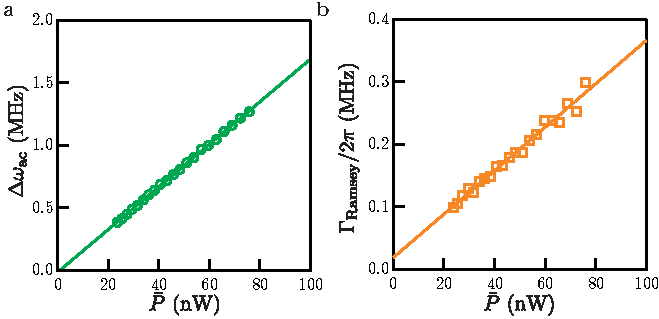
\includegraphics[width = 4.39in]{qfb_exp_chapter/chi_cal}
\end{center}
\caption[AC Stark shift and dephasing rate]{Measurements of AC Stark shift and measurement-induced dephasing rate vs. weak measurement power with linear fits.  \textbf{a} Qubit frequency shift as a function of measurement power.  Multiplying these values by the calibrated value for $2\chi$ results in the extracted value for $\bar{n}$ as a function of input power.  \textbf{b} Ramsey dephasing rate as a function of measurement power.  The offset at zero measurement power corresponds to the total environmental dephasing rate (including non-idealities such as $T_1$).}
\label{fig:chi_cal}
\end{figure*}

Many qubit and cavity parameters can be directly measured through spectroscopic means.  The cavity frequency and linewidth are measured by fitting the transmission spectrum to a Lorentzian function.  The qubit transition frequencies are measured spectroscopically.  The coherence times of the qubit are also easily measured using standard pulse sequences.  We measure $T_1 = 20$ $\mu$s using a $\pi$-pulse with a variable delay, and $T_2 = 8$ $\mu$s using a standard one-pulse spin echo sequence.

In order to determine the dispersive shift $\chi$, we use a combination of the AC Stark shift
\begin{equation}
\Delta \omega_{ac} = 2\chi \bar{n}
\label{eq:ac_stark}
\end{equation}
and measurement induced dephasing of the qubit
\begin{equation}
\Gamma_{\varphi} = 8\chi^2 \bar{n}/\kappa,
\label{eq:gamma_phi}
\end{equation}
where $\bar{n}$ is the average photon occupation of the readout cavity \cite{schusteracstark}. To measure these quantities precisely, we perform a Ramsey fringe experiment where the free evolution period between the two $\pi / 2$ pulses is modified by exciting the cavity with a fixed power $\bar{P}$ at the readout frequency $\omega_{\rm r}$. By fitting the Ramsey fringes to an exponentially decaying sinusoidal function, we measure $\Delta \omega_{ac}$ by extracting the Ramsey frequency and $\Gamma_{\varphi} = \Gamma_{\rm Ramsey} - \Gamma_2^*$ by extracting the decay constant. Here $T^\ast_{2} = 1/\Gamma^\ast_{2}$ is the decay constant of the Ramsey fringes in the absence of any photons in the cavity. This technique is significantly faster than conventional spectroscopy \cite{schusteracstark} and provides better precision in extracting $\Delta \omega_{ac}$  and $\Gamma_{\varphi}$. We repeat this process for different $\bar{P}$; since $\bar{n} \propto \bar{P}$, a plot of $\Delta \omega_{ac}$ vs $\bar{P}$ and $\Gamma_{\mathrm{Ramsey}}$ vs $\bar{P}$ gives two straight lines with slopes $m_{ac}$ and $m_{\varphi}$ (Figure. \ref{fig:chi_cal}). The ratio $m_{\varphi}/m_{ac} = 4\chi/\kappa$ then allows us to determine the dispersive shift $2\chi / 2 \pi = 1.375$ MHz. We use this value of $2\chi$ and the Stark shift data to calibrate the mean photon number $\bar{n}$ in the cavity.

\subsection{Paramp pump cancellation}

Because the strong pump for the paramp is degenerate with the measurement frequency, the cavity must be well-isolated from this signal.  Stray photons from the paramp pump which leak backwards into the cavity result in measurement-induced dephasing even in the absence of a measurement signal.  Adding additional isolation elements between the cavity and paramp will improve the isolation by approximately 20 dB per isolator, at the expense of about 1 dB of signal insertion loss in each isolator.  Because we aim to realize a highly efficient measurement apparatus, we must take great pains to minimize the signal loss between the cavity and paramp.

Due to the reflection geometry of the paramp, we require at least one circulator to separate input and output modes.  Furthermore, from the discussion in section \ref{s:jpa_perf}, the pump power must be about 40 dB larger than the input signal, implying that 40 dB of isolation (two isolator elements) would still result in a large stray signal in the cavity, on the order of our largest measurement signal.  We aim to make the dephasing due to the stray pump leakage much smaller than the intrinsic environmental dephasing rate $\Gamma_\mathrm{env}$.  From \eqref{eq:gamma_phi}, for $\Gamma_\mathrm{leakage} < 0.1 \Gamma_\mathrm{env}$, that places an upper limit on the photon number in the cavity $\bar{n}_\mathrm{leakage} < 0.007$, or a power incident on the cavity of less than $P_\mathrm{leakage} < -175$ dBm.  Typical pump powers are on the order of -90 dBm, implying a need for about 80 dB of isolation.  The $\sim$4 dB loss from using four circulators would imply a maximum measurement efficiency $\eta = 0.4$, much smaller than unity.

To avoid this issue, we use two circulators rather than four, providing $\sim$40 dB of isolation.  To achieve the additional isolation needed, we connect another signal line to the third port of the first circulator as shown in Figure \ref{fig:full_schem}.  At room temperature, we tap off a small portion of the paramp pump using a directional coupler, and pass this signal through a variable attenuator and a phase shifter and inject it into this extra signal line.  The circulator directs this signal back towards the strongly coupled port of the cavity and is thus co-propagating with any pump leakage.  By carefully tuning the attenuation and phase shift with the paramp pump energized, this extra \textit{pump cancellation signal} interferes destructively with the leakage signal.

The pump cancellation attenuation and phase is tuned by hand while Ramsey oscillations of the qubit are continuously measured, using the AC Stark shift of the qubit as a very sensitive power meter.  When the AC Stark shift is nearly zero compared to the value measured with the pump off, the pump signal has been well cancelled.  This is also reflected in the dephasing rate extracted from the same experiment.  Due to the linearity of the microwave injection lines and the fact that the pump cancellation signal is split from the pump after the attenuator which controls the pump amplitude, once the attenuation and phase are set for the pump cancellation signal, the cancellation remains perfect even when the pump amplitude is adjusted.  Changing the pump frequency requires re-tuning the cancellation signal.

Shortly after this experiment concluded, an alternative pumping technique known now as ``double-pumping'' came into favor, where the paramp is driven by two strong pump tones symmetrically detuned above and below the center frequency \cite{PhysRevB.79.184301}.  This technique significantly eases the issue of pump cancellation, as the drive tones can be detuned by several hundred megahertz, ensuring that the total power leaking back towards the cavity is well-filtered by the cavity response function.  For details on the experimental implementation of this technique, see reference \cite{Weber2014a}.


\subsection{Dumb signal cancellation}

\begin{figure*}
\begin{center}
	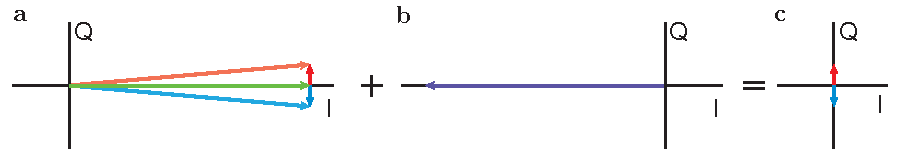
\includegraphics[width = 6in]{qfb_exp_chapter/dumb_sig}
\end{center}
\caption[Dumb signal cancellation]{\textbf{a} IQ vector diagram showing the coherent state vectors for the ground state (pale blue) and excited state (pale red), and the decomposition of those vectors into the qubit state components (dark red and dark blue) and the component which contains no qubit state information (green), the dumb signal.  \textbf{b} A coherent tone phase-shifted by 180 degrees with identical amplitude to the dumb signal.  \textbf{c} The coherent addition of these vectors results in only the pure qubit state component without the large extra signal power associated with the dumb signal.}
\label{fig:dumb_sig}
\end{figure*}

Because this experiment is conducted in the limit where $\chi \ll \kappa$, the phase shift between the output signals is quite small.  Thus, to achieve large signal-to-noise ratio in a projective measurement of the qubit, the cavity occupation $\bar{n}$ must be increased to separate the qubit state histograms.  In the IQ plane, we can decompose this signal into two components: the component in the quadrature which contains qubit state information, and the component in the other quadrature which will be squeezed by the parametric amplifier.  This vector decomposition is shown in Figure \ref{fig:dumb_sig}.  The vast majority of the power in the signal is in the quadrature which contains no information about the qubit state; we call this the \textit{dumb signal} as it ``knows nothing'' about the qubit state.  Ideally, the paramp will squeeze this quadrature away.  However, the alignment between the paramp and signal phase is never perfect, and this extra power can cause input compression if the phase angle is slightly misaligned and part of this power ends up in the amplified quadrature.

\begin{figure*}
\begin{center}
	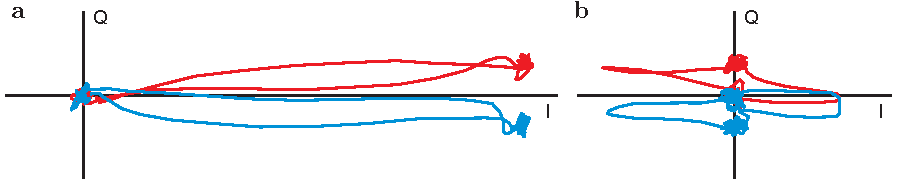
\includegraphics[width = 6in]{qfb_exp_chapter/dumb_sig_exp}
\end{center}
\caption[Dumb signal cancellation data]{\textbf{a} Measured IQ trajectories for the ground state (blue) and excited state (red), showing the large dumb signal component.  Axes have a square aspect ratio with arbitrary units.  Trajectories start and end at the origin, so the loops correspond to the ring-up and ring-down of the resonator.  \textbf{b} The same trajectories with the addition of the optimized dumb signal cancellation path.  The separation at steady-state is the same, but the large extra signal power has been cancelled.  Axes have the same scaling as in \textbf{a}.}
\label{fig:dumb_sig_exp}
\end{figure*}

We avoid this problem by tapping off a portion of the qubit measurement signal at room temperature using a directional coupler, passing this signal through a variable attenuation and phase shifter, and adding it to the paramp pump signal.  With the paramp pump off, the amplitude and phase shift of this \textit{dumb signal cancellation signal} is adjusted by hand to draw the IQ histograms for the qubit ground and excited states back towards the origin.  This optimization is relatively easy compared to the paramp pump cancellation tuning procedure, as the cancellation does not need to be particularly precise.  Actual measured IQ trajectories for the ground and excited states are shown in Figure \ref{fig:dumb_sig_exp}a.  This type of plot is used to adjust the amplitude and phase of the dumb signal cancellation signal until the steady-state trajectories are centered at the origin, as shown in Figure \ref{fig:dumb_sig_exp}b.  With the dumb signal component well cancelled, small phase mismatches between the signal and paramp pump no longer result in paramp compression during projective readout.  Just like for pump cancellation, because of the circuit topology and the linearity of the intermediate circuit components, once the amplitude and phase are adjusted, the cancellation works well for any pulse amplitude or duration.  There are still some transient effects during ring-up and ring-down due to the finite resonator bandwidth, but these are not important for good steady-state readout performance.

\subsection{Detector and measurement efficiency}\label{s:det_meas_eta}


The overall measurement efficiency relevant for feedback is given by $\eta = \eta_{\mathrm{det}} \ \eta_{\mathrm{env}}$. The first term $\eta_{\mathrm{det}}$ accounts for the noise added by the amplification chain. To measure this noise, we use the qubit-cavity system as a calibrated signal power source. As discussed in section \ref{s:chi_cal}, we can excite the cavity with a precise average photon occupation $\bar{n}$. This corresponds to an RMS power radiated from the cavity $P_{\mathrm{rad}}= \hbar\omega_{r} \kappa \bar{n}$, where $\omega_{r}$ is the frequency of excitation. We send this signal to the paramp and measure the signal-to-noise ratio (SNR) at the output. This allows us to extract the noise floor of the entire measurement chain referred to the output plane of cavity, which includes dominant contributions from the signal loss between the cavity and paramp and imperfections in the paramp itself, as well as a smaller contribution from the noise added by the HEMT amplifier. 

The noise floor referred to the input of the amplification chain is given by $P_{\rm n} = \hbar \omega_{r}B/\eta_{\rm det}$, where $B$ is the integration bandwidth (in Hz).  The signal-to-noise ratio can then be expressed as
\begin{equation}
\mathrm{SNR}=\frac{P_\mathrm{rad}}{P_\mathrm{n}}.
\end{equation}
Substituting in the expressions for $P_\mathrm{rad}$ and $P_\mathrm{n}$, we can solve for the detector efficiency in terms of the measured SNR, yielding the expression
\begin{equation}
\eta_{\rm det}=\frac{{\rm (SNR)}}{   \bar{n}} \frac{B }{ \kappa}.
\end{equation}
This definition of $\eta_{\rm det}$ is consistent with phase-sensitive operation of the paramp and measures the departure from the best SNR we could possibly obtain when amplifying at the quantum limit. We measure the SNR for a range of frequencies within the paramp bandwidth and extract an average detector efficiency $\eta_{\rm det}=0.46$.  Using cryogenic switches, separately measure the attenuation between the cavity and the paramp to be roughly 2.5 dB, implying that signal attenuation is the dominant source of reduction in detector efficiency.

 The final contribution to the overall measurement efficiency is due to environmental decoherence via pure dephasing. The efficiency $\eta_{\mathrm{env}} = (1+\Gamma_{\mathrm{env}} / \Gamma_{\varphi})^{-1}$ characterizes how much of the total dephasing is due to measurement. In principle we could improve this efficiency by increasing $\bar{n}$ (and thus $\Gamma_{\varphi}$), but there are two practical constraints. First, the measurement must be weak enough that it is not projective on the timescale of the Rabi period $\Omega_{\rm R}^{-1}$, ensuring the qubit evolution remains mostly oscillatory. Second, the required feedback bandwidth increases with $\Gamma_{\varphi}$. Since the effective feedback bandwidth is fixed by the measurement chain, the feedback efficiency $D$ decreases with increasing measurement strength if $\Gamma_{\varphi}$ becomes too large.  Dephasing due to low frequency noise does not affect the feedback efficiency because the system can track any slow variations in the qubit frequency (and consequently in the Rabi frequency). Hence, we set $\Gamma_{\mathrm{env}} = 1/T_2$ measured from echo experiments giving us $\Gamma_{\mathrm{env}}/2\pi = 0.02$ MHz, and $\eta_{\mathrm{env}}=0.87$.  This definition includes the dephasing contribution from qubit relaxation ($\Gamma_1 / 2$).


\subsection{Projective measurement and qubit temperature}

Because we realize a high-quantum-efficiency measurement chain, making a faithful projective measurement is simply a matter of acquiring sufficient SNR to separate the histograms corresponding to the ground state and excited state in a time much shorter than the qubit relaxation time.  We use a photon number $\bar{n} = 11$ and an integration time of 800 ns to acquire well-separated histograms.  This integration time is not negligible compared to $T_1$, so the fidelity of the readout is primarily constrained by this.  For most experiments of interest, this reduction in fidelity from unity is not important so long as the fidelity remains high, on the order of 90\% or more, such that SNR remains high.  A discussion of how imperfect readout fidelity is calibrated out of the results appears in section \ref{s:qst_cal}.

\begin{figure*}
\begin{center}
	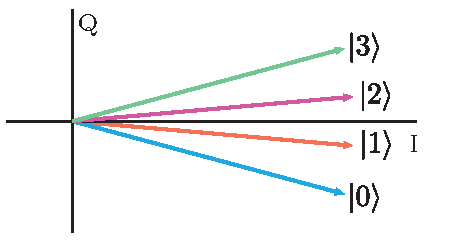
\includegraphics[width = 3in]{qfb_exp_chapter/qutemp_IQ}
\end{center}
\caption[IQ vectors for multi-state readout]{IQ vector diagram showing the coherent state vectors for the first four qubit states.  By aligning the phase of the measurement signal to be roughly centered on the phase between the states $\ket{1}$ and $\ket{2}$, the total phase shifts are small enough to be measured simultaneously without compressing the paramp.}
\label{fig:qutemp_IQ}
\end{figure*}

Since the cQED system is optimized to the weak measurement regime where the phase shift between qubit states is small, it is possible to measure more than just the $\{ \ket{0},\ket{1} \}$ manifold.  An IQ diagram showing the coherent state vectors corresponding to several qubit states in an idealized representation is shown in Figure \ref{fig:qutemp_IQ}.  Each qubit state above $\ket{1}$ shifts the resonant frequency of the cavity by (approximately) an additional amount $2 \chi$, such that the signal phase can be adjusted to observe the readout histograms for several states simultaneously.  The actual shift for the higher states is somewhat smaller than $2 \chi$, but this detail is not important here.

\begin{figure*}
\begin{center}
	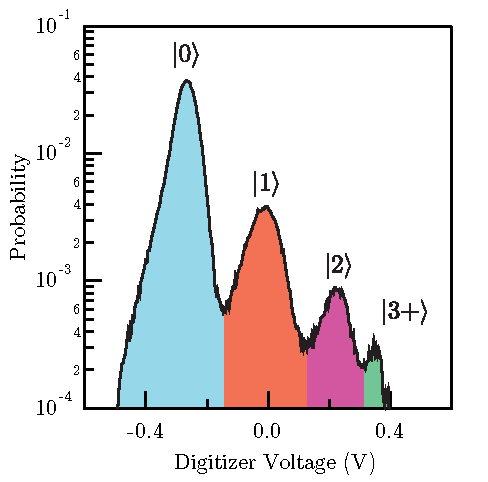
\includegraphics[width = 3.25in]{qfb_exp_chapter/qutemp}
\end{center}
\caption[Qubit temperature histograms]{Readout histograms showing non-trivial occupation of energy levels above the ground state.  The state occupations are $P_0 = 0.83$, $P_1 = 0.13$, $P_2 = 0.03$, and $P_{3+} = 0.01$.}
\label{fig:qutemp}
\end{figure*}

Due to the high single-shot fidelity of the readout, we can measure the temperature of the qubit in thermal equilibrium simply by measuring an ensemble of qubits with no explicit state preparation.  After each measurement, we wait for approximately $10 \ T_1$ to allow the qubit to re-thermalize.  Histograms of this measurement are shown in Figure \ref{fig:qutemp}.  The distribution of state occupation probabilities does not obey a Boltzmann distribution, so it is not precisely a thermal state.  However, if we approximate the system by only considering the first two levels, we can approximate the distribution as thermal and assign a temperature of approximately 140 mK, much higher than the thermal temperature of the dilution refrigerator (about 30 mK).  This type of spurious excited state population has been observed in other experiments \cite{fluxqb,Geerlings2013,Jin2014} and was common for superconducting qubits of this era.  It is now reasonably well understood that that these large spurious populations are due to quasiparticle excitations created by stray infrared photons.  Enhancing the degree to which the qubits are shielded from stray light has been shown to enhance coherence times and significantly reduce the spurious thermal population \cite{Barends2011}.

Because the readout is QND, we can use the readout itself to artificially create an ensemble of qubits which are perfectly prepared in the ground state through post-selection.  The protocol is to insert a projective measurement pulse at the start of the experiment, and then perform the experiment as usual.  When the data is analyzed, any experimental records in which the qubit did not start in the ground state are thrown out, creating a post-selected ensemble in the ground state at the cost of throwing away the fraction of the data corresponding to the spurious excited state population.  The first application of this post-selection cooling technique was the subject of a separate work published in Physical Review Letters \cite{fluxqb}.  The technique of purifying ensembles using post-selection and the QND nature of the cQED readout is quite useful for removing experimental imperfections in general, and is applied in numerous places in the work in this thesis.

\subsection{Quantum state tomography}\label{s:qst_cal}

Fully reconstructing the quantum state of a qubit requires measuring an ensemble of identically-prepared qubits along at least three different qubit measurement axes.  The cQED measurement naturally probes the qubit state in the $\sigma_z$ basis, so an ensemble of measurements provides $\xpec{\sigma_z}$.  To measure $\xpec{\sigma_x}$ ($\xpec{\sigma_y}$) we must first rotate the qubit state by an angle $\pi/2$ about the $\hat{y}$ ($-\hat{x}$) axis (respectively).  These expectation values define the Bloch vector components and thus the density matrix of the qubit state.

To ensure accurate tomographic results, the measurement and qubit manipulation pulses must be precisely calibrated.  After single-shot measurement is tuned up (mostly a matter of aligning the signal and paramp phase and tuning the measurement power and integration time), we can precisely calibrate a $\pi$-pulse by adjusting the pulse amplitude until we maximize $P(\ket{1})$.  Because of the finite measurement fidelity due to qubit relaxation during readout, $P(\ket{1})$ will never go all the way to 1; this implies that even if we prepare the excited state, we would not measure $\xpec{\sigma_z} = -1$.  This effect is easy to correct for by measuring the values of $P(\ket{1})$ for the ground state ($P_g$) and the excited state ($P_e$).  Then, when we measure $P(\ket{1})$ for an experimental ensemble, we re-scale it as 
\begin{equation}
P(\ket{1})' = \frac{P(\ket{1}) - P_g}{P_g + P_e}.
\end{equation}
Since $P(\ket{2+})$ is not negligible, we use post-selection to eliminate experimental records where the qubit was found outside the $\{ \ket{0},\ket{1} \}$ manifold.  Because none of the control pulses are resonant with any transition involving the higher qubit states, this post-selection essentially eliminates the effect of thermal excitation out of the $\{ \ket{0},\ket{1} \}$ manifold on the tomographic reconstruction of the target state, improving both the tomographic quality as well as the quality of the measured state itself.

We utilize a series of combination pulses to calibrate the $\pi/2$ pulses on $\hat{y}$ and $-\hat{x}$.  We calibrate the amplitude of the $\pi/2$ pulses by adjusting the pulse amplitudes until $P(\ket{1})' = 0.5$ for each.  We verify that the $\pi$ and $\pi/2$ pulses are balanced by measuring $P(\ket{1})'$ for a $\pi$ pulse immediately followed by a $\pi/2$ pulse, and ensuring that $P(\ket{1})'$ is still maximized for $\pi$ while $P(\ket{1})' = 0.5$ for the bare $\pi/2$ and the $\pi + \pi/2$ sequence.  We then check the orthogonality of the $\hat{y}$ and $-\hat{x}$ axes by measuring two sequences that have two $\pi/2$ pulses in sequence, one on each axis.  Deviations from $P(\ket{1})' = 0.5$ indicate that the two axes are not perfectly orthogonal.  We utilize the vector generator's built-in quadrature skew correction feature to null this effect to the couple-percent level.  This entire optimization sequence is somewhat challenging, as the quadrature skew correction also effects the balance of the I and Q inputs, requiring the absolute and relative amplitudes of the pulses to be re-adjusted.  All in all this procedure is iterated a few times until all of the pulses are in balance; at this point, the system is essentially stable aside from overall RF level fluctuations, which are easily controlled.  In reality, all of these pulses are programmed into a single AWG sequence along with a given experiment of interest, thus monitoring the quality of tomography during the experiment.

We make no attempt to include any error amplification or self-consistency techniques in the calibration sequence \cite{Chow2009,Merkel2013,Blume-Kohout2013}; as such, this calibration technique is somewhat ``rough and ready,'' but insufficient to achieve calibration better then the few percent level.  Because the measurement efficiency in this experiment is about 0.4 and the feedback efficiency $D$ and thus the stabilized Bloch vector amplitude is constrained to be less than $\sqrt{\eta} = 0.63$, a few percent error in the pulse calibrations is tolerable to reasonably well characterize $D$.  Contemporary experiments in the lab utilize more sophisticated calibration techniques, including error amplification by repeated pulses.  Furthermore, we now typically use single-sideband modulators instead of IQ mixers, sidestepping the issue of quadrature skew correction entirely and allowing full Bloch sphere control of one qubit from a single AWG channel by utilizing finite-frequency pulses.

\subsection{Loop delay}\label{s:loop_delay}

The quality of the feedback control will depend on the total round trip delay time $\tau_{\rm delay}$ between a measurement signal leaving the cavity and the corresponding feedback correction entering the cavity.  This delay can be broken into two pieces: the delay in the microwave-frequency part of the system and the delay in the low-frequency part of the system.  The microwave delay includes the propagation time through the transmission lines into and out of the experiment, and also implicitly includes the bandwidth of the microwave cavity and paramp.  Because the cavity has a relatively large bandwidth, $1/\kappa \sim 10$ ns, and only contributes to the measured value of $\tau_{\rm delay}$ at the few percent level.  We measure the microwave delay by injecting a $\pi$-pulse into the fridge while the qubit is being weakly measured.  We tap off a portion of the voltage envelope that drives the IQ mixer, and feed it to the I channel of the digitizer (properly accounting for extra cable length for signal routing).  We then measure the delay between the arrival of this pulse at the digitizer and the arrival of the leading edge of the shift in resonator phase on the Q channel, resulting in $\tau = 200$ ns ($\pm$ 10 or 20 ns or so).  Measuring the delay in the low-frequency portion of the measurement chain is a straightforward matter of measuring pulse propagation delay using an oscilloscope, a total delay of about 80 ns, for a grand-total loop delay of about 280 ns.

\subsection{Feedback strength calibration}

The theory for feedback stabilization is expressed using a dimensionless feedback strength parameter $F$ which takes into account all of the relevant gain stages in the system.  To compare to theory, we must calibrate the feedback loop to determine the gain in normalized units.  First, we use the digitizer to measure the full voltage swing $\Delta V$ in the output of the demodulation setup between the qubit being in the ground state vs. the excited state for a given measurement strength.  We use post-selection on an initial and final strong measurement pulse to prepare an ensemble of very pure ground and excited-state preparations, then integrate an intermediate weak measurement pulse to get $\Delta V$ (see section \ref{s:weak_meas} for additional details on this technique).

We use a low-frequency signal generator to create a pure sine wave at $\Omega_r$ with peak-to-peak amplitude $\Delta V$, and feed this signal into the feedback circuit in place of the demodulator output.  By measuring the voltage swing at the output of the feedback loop, where the feedback signal is re-combined with the voltage which sets the Rabi frequency, we measure the gain of the feedback loop.  Because we know the voltage applied at this point to set a particular Rabi frequency $\Omega_r$, we can express the feedback gain as the non-dimensional ratio of the voltage scale of the feedback correction and the voltage which sets the Rabi frequency $\Omega_r$.










